\chapter{Lost Lepton Background}
\label{chap:lostlep}

A second source of background comes from events where a genuine prompt lepton is produced
from the decay of a $W$ boson. While the tight lepton veto employed in the analysis 
aims to eliminate as many of these events as possible, a significant number still enter
the signal regions because the lepton gets ``lost''. This can happen for a number
of reasons, such as the lepton being outside of the acceptance window (i.e. it is too forward
 or the \pt is too small) or not being isolated, or the reconstruction algorithms
failing to identify the candidate as a lepton. 

Generally the energy of the lepton is still
accounted for (making ``lost'' a bit of a misnomer), so there is no fake \ptmiss from the lepton. 
However, there is real \ptmiss from the neutrino from the $W$ decay, and this is often enough
to allow the event to enter the signal region. The dominant production mechanisms for the lost
lepton background are \wjets and \ttbar production, but there are also smaller contributions
from rarer processes such as single top, $\ttbar W$, $\ttbar Z$, $\ttbar H$, and $tt\bar{t}\bar{t}$.

The lost lepton background is estimated in a data-driven way using a control sample of events
where there \emph{is} a reconstructed lepton. Section~\ref{sec:llep_pred} describes how this
is done in each $(\Ht, \Nj, \Nb)$ topological region, Sec.~\ref{sec:llep_mt2} explains the method
for extrapolating along the \mttwo dimension, and Sec.~\ref{sec:llep_syst} lists the systematic
uncertainties assessed on the final estimate.

\section{Prediction from single lepton control regions}
\label{sec:llep_pred}

The lost lepton estimate is performed with single lepton control region, described in detail 
in Sec.~\ref{sec:crsl}. It mainly inverts the  lepton veto employed in the signal regions,
but with the additional requirement that $M_\mrm{T}(\mrm{cand},\vMet)<100\GeV$, in order
to reduce signal contamination. All individual processes (\wjets, \ttbar, etc.) are summed
for the purposes of computing the estimate (i.e. there is only a single transfer factor for all
processes combined).

Data vs. MC comparisons of the main analysis kinematic variables in the baseline single lepton
control region are shown in Fig.~\ref{fig:llep_crplots}. As with the dilepton control region,
there is some level of disagreement between data and MC, but this is to be expected. The 
estimate is again primarily data driven, and these disagreements generally do not affect the
final estimate. As described below, in high \Nj regions MC is used to extrapolate along the
\Nb dimension. To account for known $\ttbar+\mrm{heavy flavor}$ mismodeling in MC, we correct the MC 
with a reweighting procedure described in Sec.~\ref{sec:llep_ttbb}.

\begin{figure}[ht]
  \begin{center}
    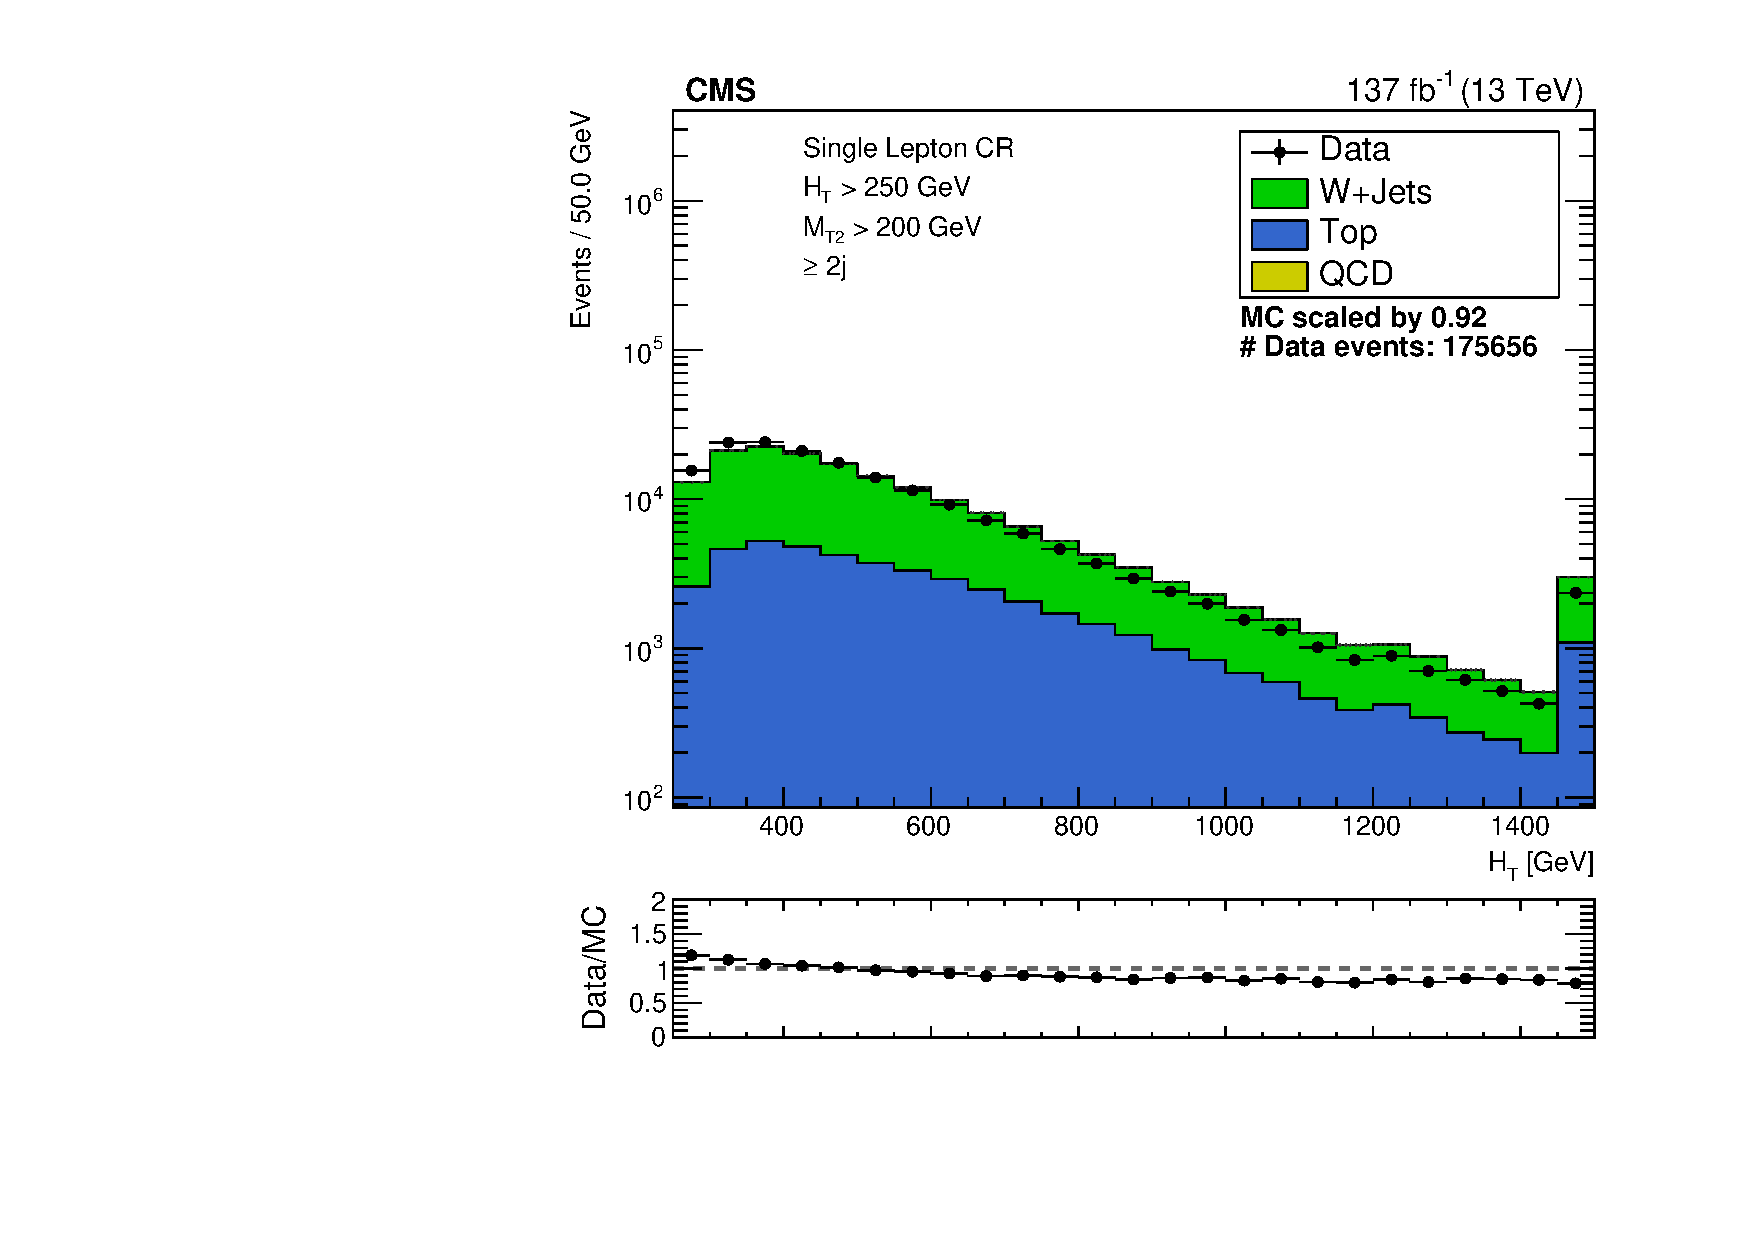
\includegraphics[width=0.47\textwidth]{figs/llep/crslbase_ht.pdf}
    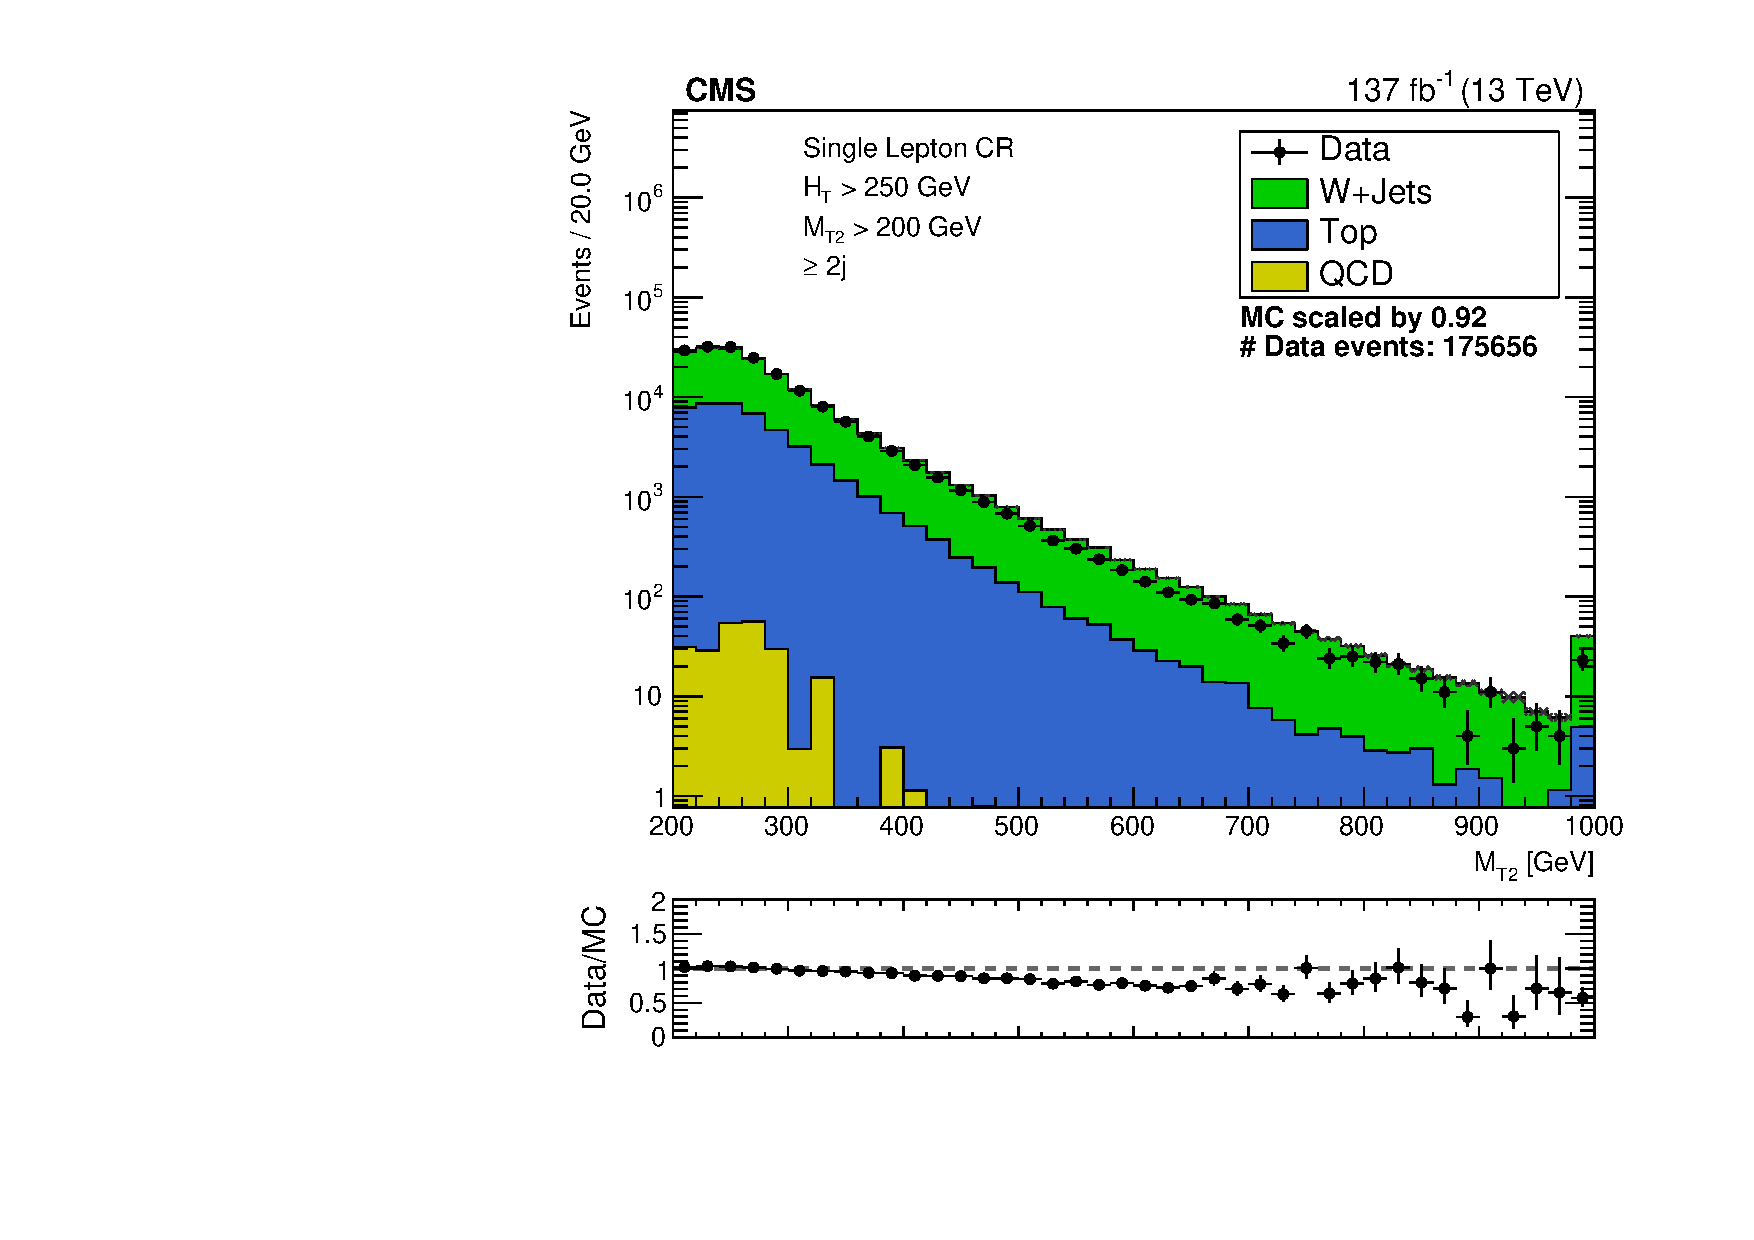
\includegraphics[width=0.47\textwidth]{figs/llep/crslbase_mt2.pdf} \\
    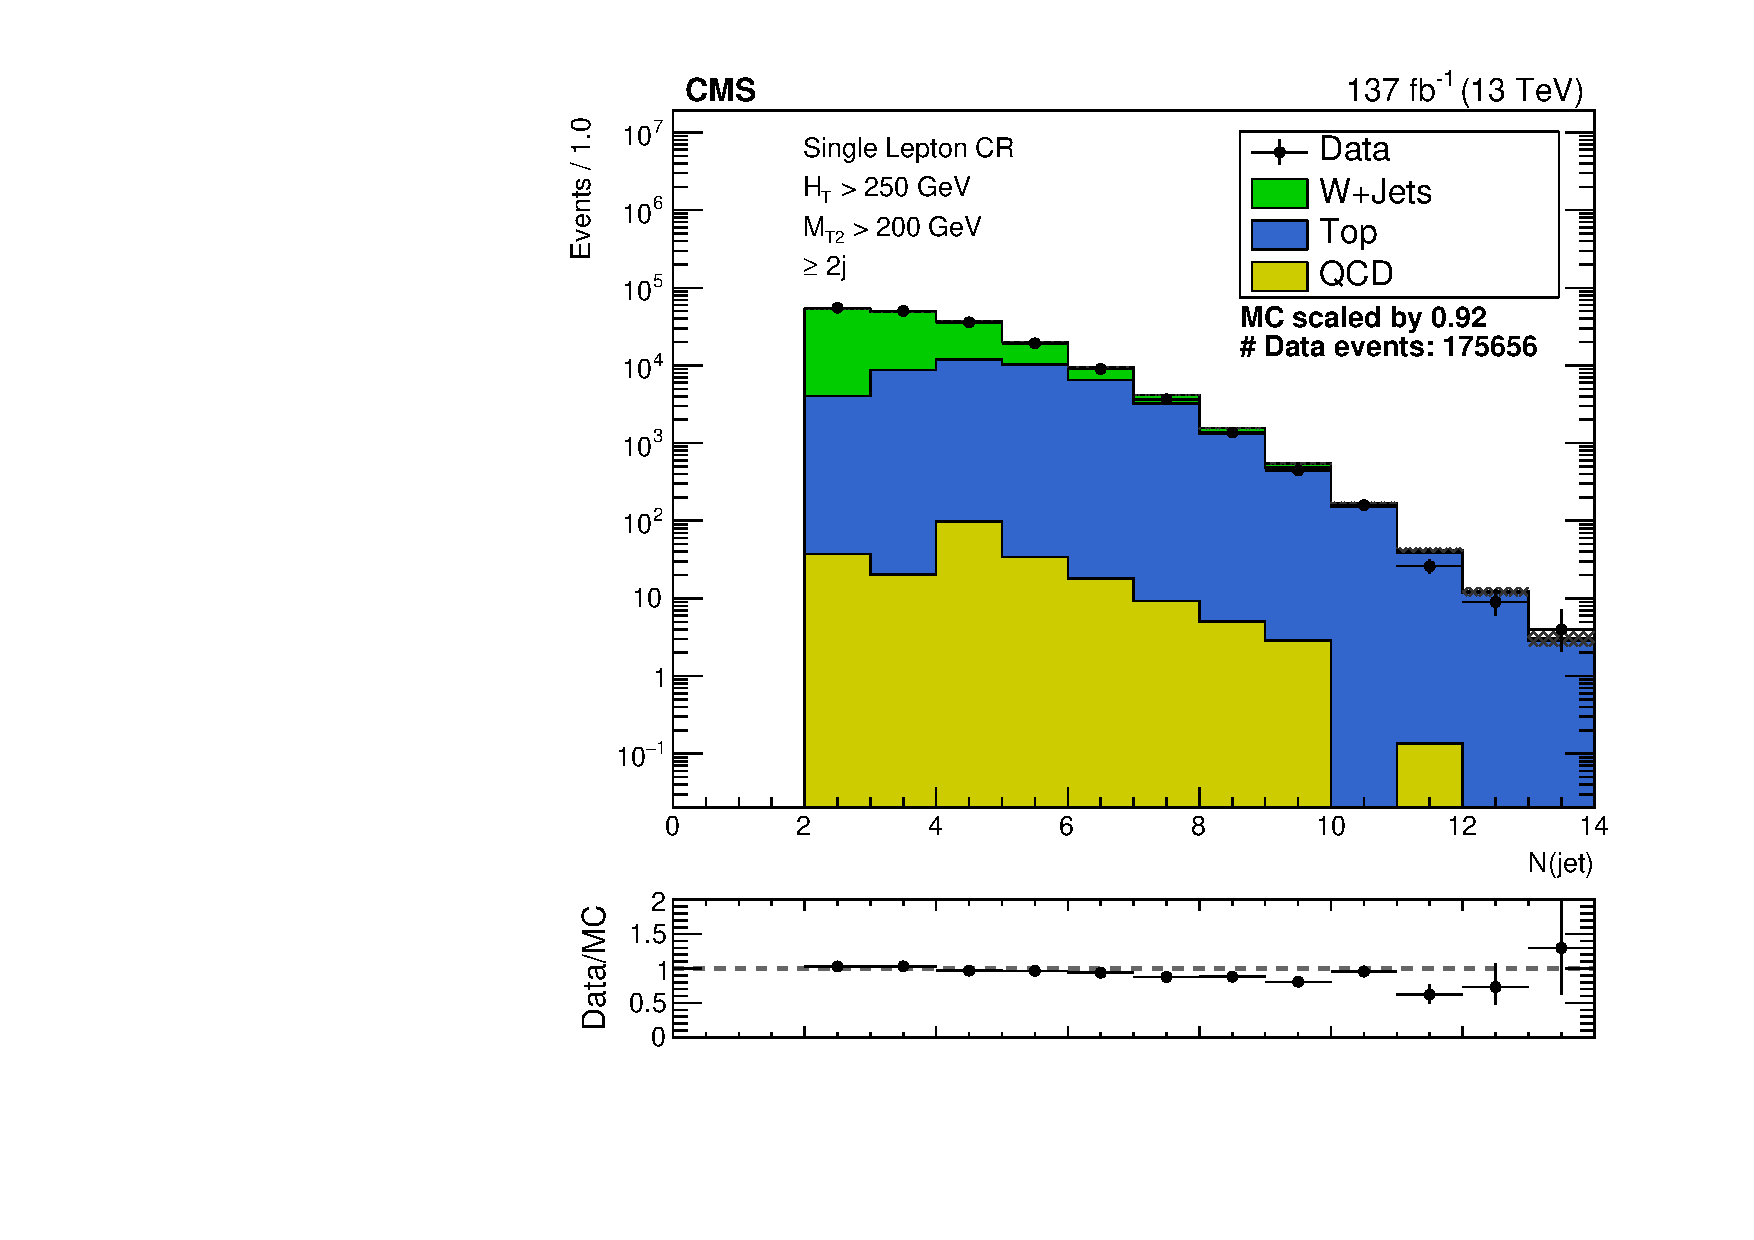
\includegraphics[width=0.47\textwidth]{figs/llep/crslbase_nJet30.pdf}
    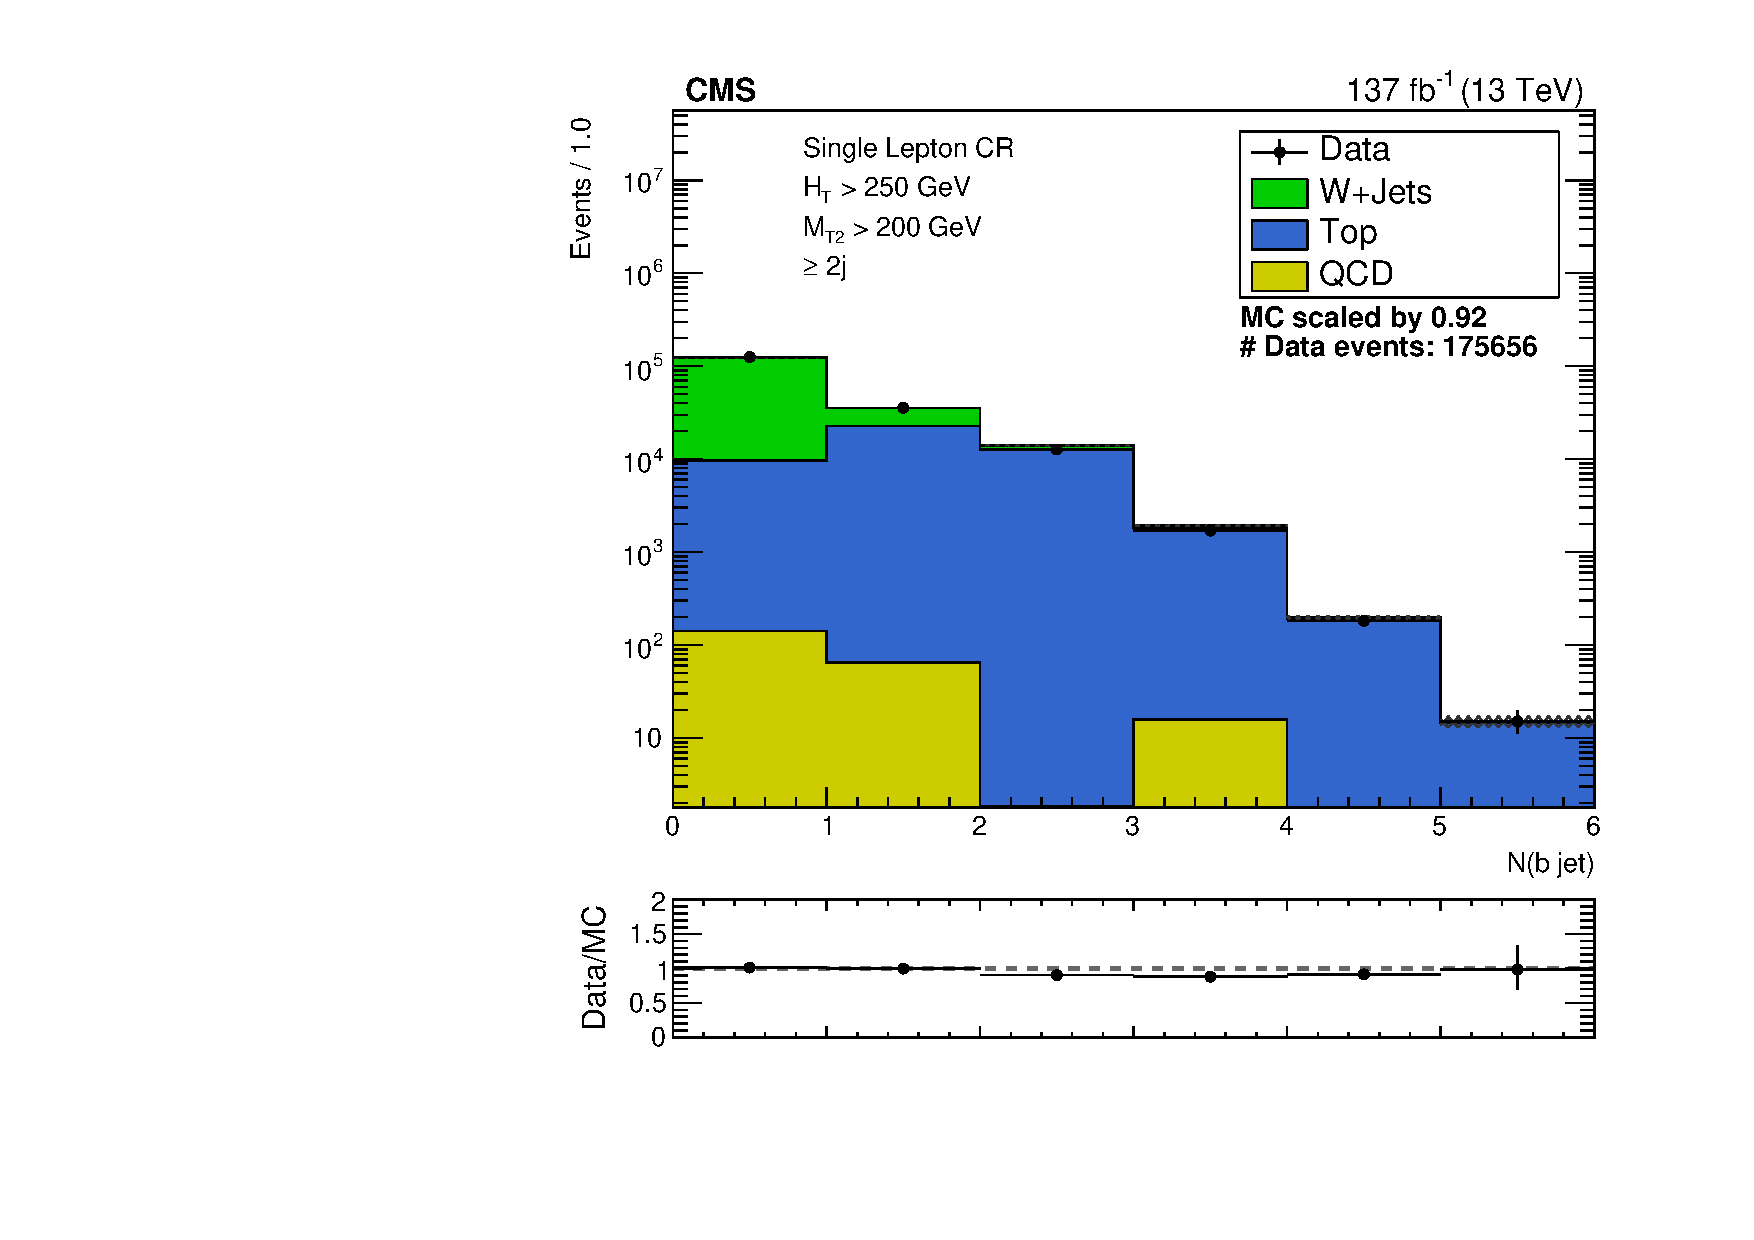
\includegraphics[width=0.47\textwidth]{figs/llep/crslbase_nBJet20.pdf} \\
    \caption{Data vs.\ MC comparisons in the baseline single lepton control region, for $\Nj\geq2$.
      From left to right, top to bottom, the variables
      plotted are \Ht, \mttwo, \Nj, and \Nb.
            }
    \label{fig:llep_crplots}
  \end{center}
\end{figure}

As with the \znunu estimate,
the lost lepton estimate is first performed in each $(\Ht,\Nj,\Nb)$ topological region, integrated
over \mttwo (for the monojet region, the \Ht dimension is equivalent to $\vSS{p}{T}{\mrm{jet1}}$,
so there is no integration and the estimate is performed in each analysis bin). For all regions
with 7--9 or $\geq$10 jets and $\geq$1 b tag, an inclusive control region with $\geq$7 jets and 1--2 b tags
is used, to avoid low statistics and higher signal contamination in regions with high jet and b-jet multiplicity.
Similarly, rgions with either 7--9 or $\geq$10 jets and 0 b tags are all predicted using control region bins
with $\geq$7 jets and 0 b tags, due to low control regions statistics in regions with $\geq$10 jets.

Fig.~\ref{fid:llep_njextrap} shows \Nj distributions for data and MC in the $\geq$7 jet region, for both $\Nb=0$
and $\Nb\geq1$. Good agreement is observed, justifying the use of MC to extrapolate into the $\geq$10 jet regions
as described above. For the $\Nb$ distribtions, agreement is not as good, so a reweighting is performed to correct
MC as described in the following section.

\begin{figure}[ht]
  \begin{center}
    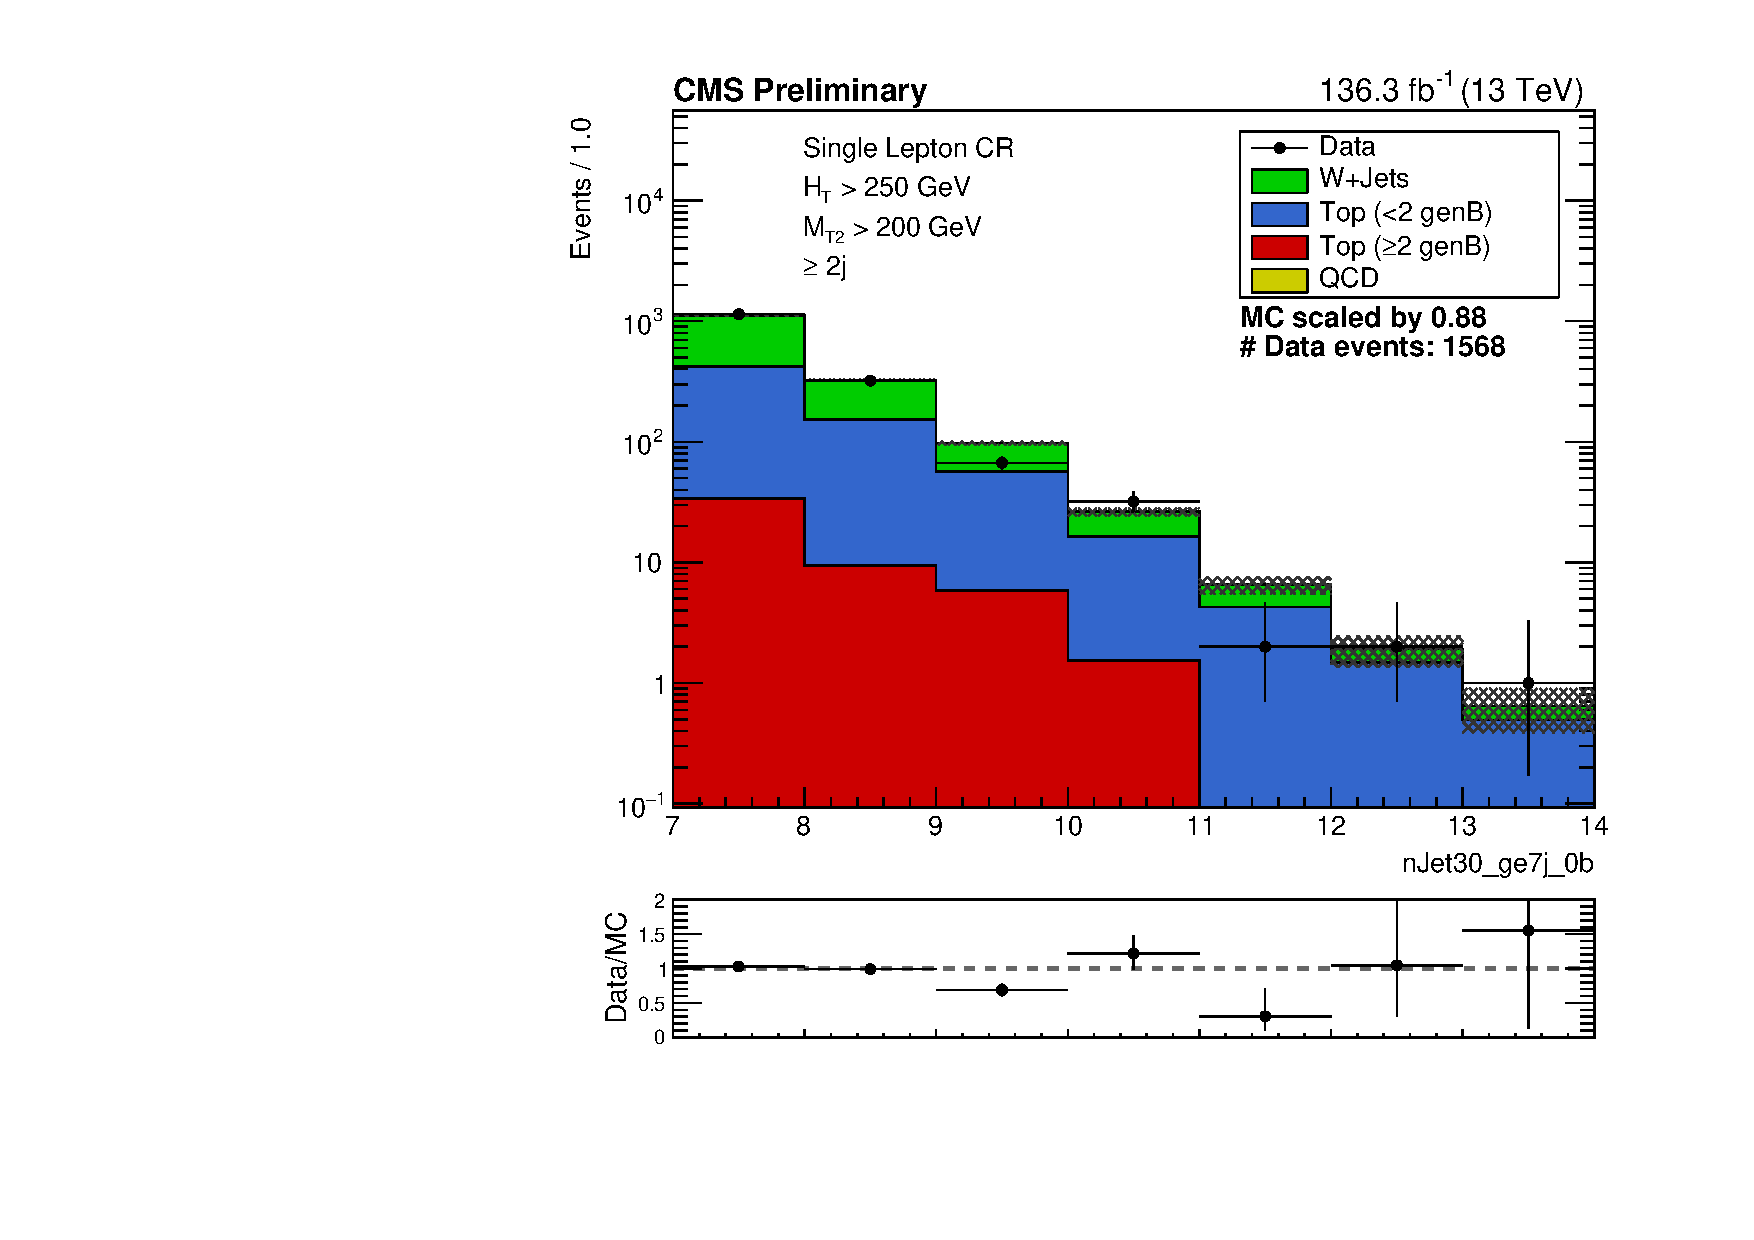
\includegraphics[width=0.47\textwidth]{figs/llep/crslbase_nJet30_ge7j_0b.pdf}
    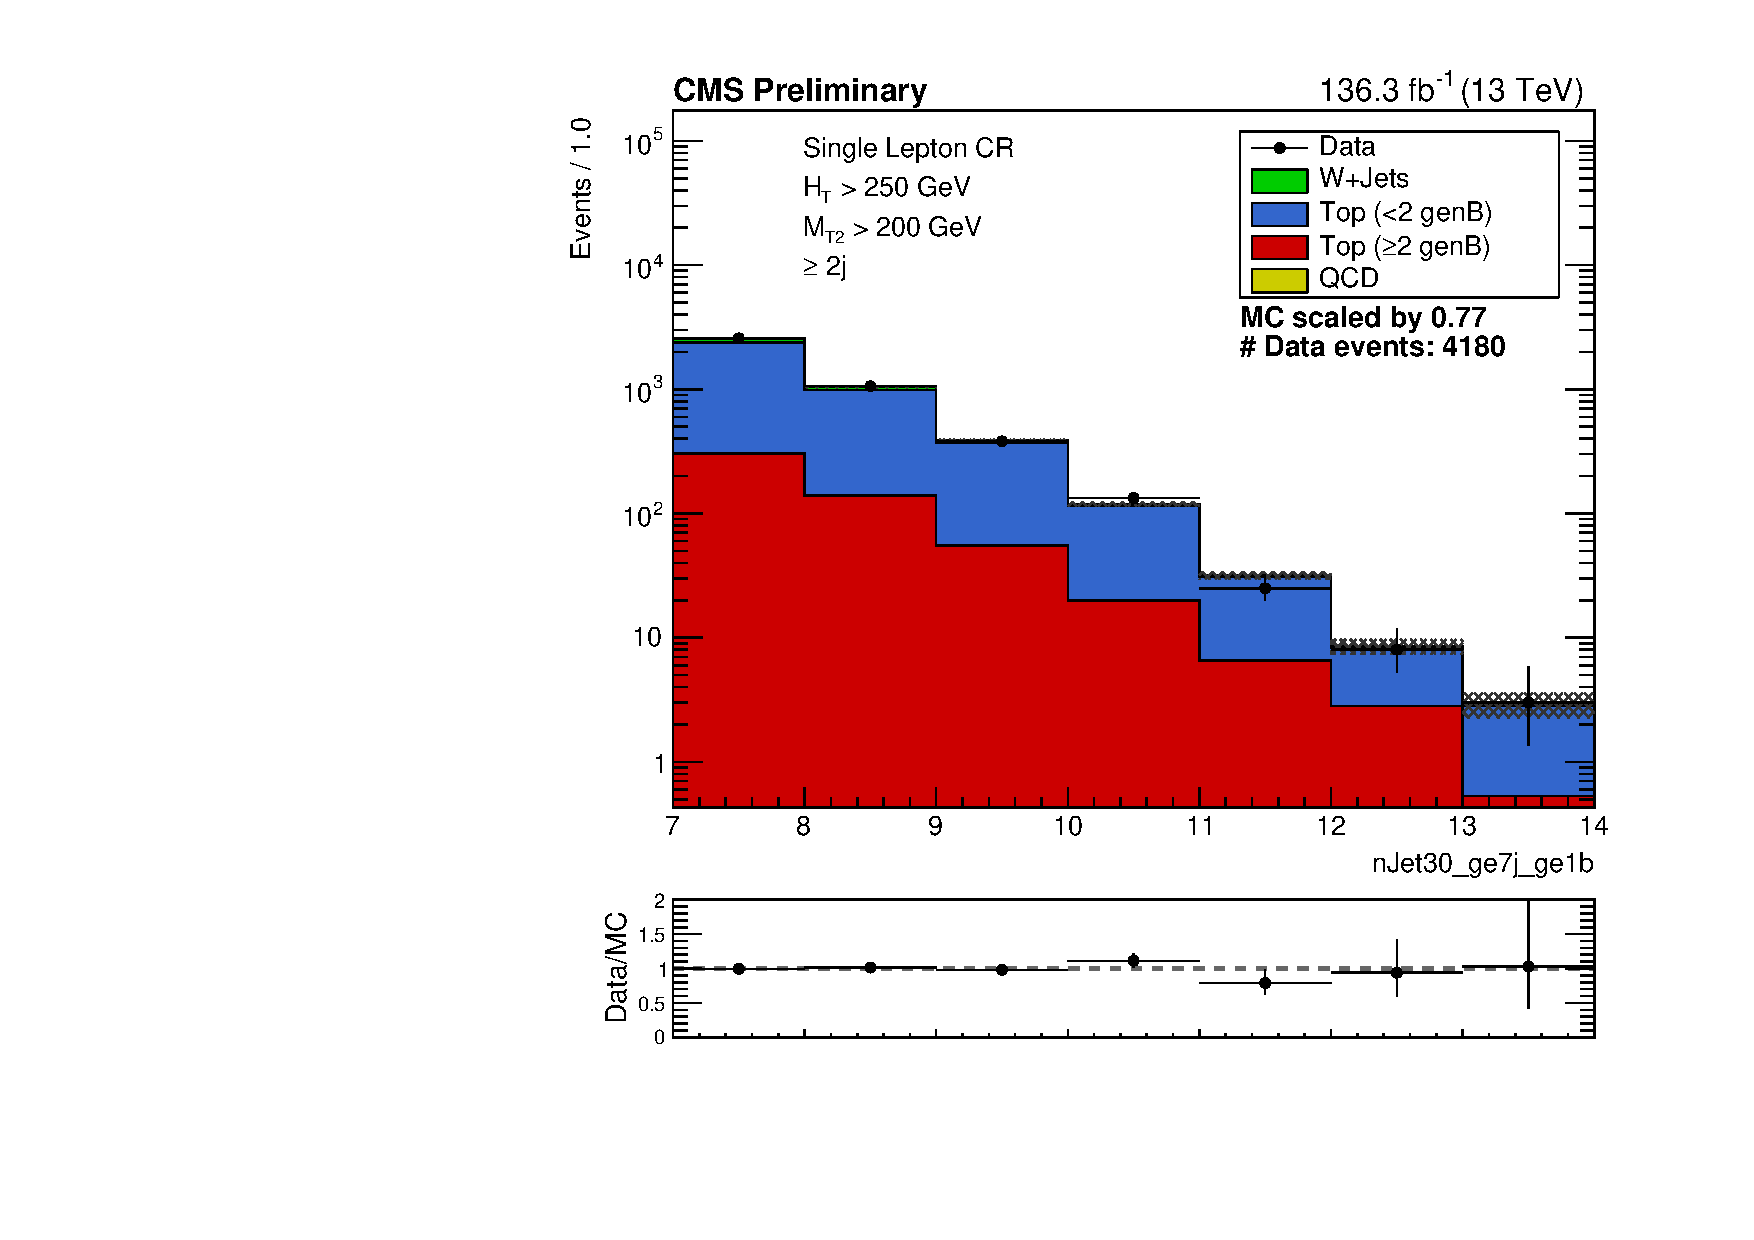
\includegraphics[width=0.47\textwidth]{figs/llep/crslbase_nJet30_ge7j_ge1b.pdf}
    \caption{Data vs.\ MC \Nj comparisons in the baseline single lepton control region with $\Nj\geq7$,
      for $\Nb=0$ (left) and $\Nb\geq1$ (right). Agreement is sufficient to justify using MC to extrapolate
      along the \Nj dimension for high-\Nj regions.
            }
    \label{fig:llep_njextrap}
  \end{center}
\end{figure}

For regions with $\Ht>1500\GeV$, all events with
$\mttwo>200\GeV$ are used in the control region even though the signal region starts at $\mttwo>400\GeV$.
Once the per-topological region estimate is done, a hybrid approach using both data and MC is
used to extrapolate along the \mttwo dimension, as described in Sec.~\ref{sec:zinv_mt2}.

The final estimate in each $(\Ht,\Nj,\Nb,\mttwo)$ signal region can then be summarized as
\be\label{eq:zinv_est}
N_{\mrm{LL}}^\mrm{SR} = N_\mrm{1\ell}^\mrm{CR}(\Omega)\; R_\mrm{MC}^{0\ell/1\ell}(\Omega)\;
k_\mrm{LL}(\mttwo|\Omega),
\ee
where
\begin{itemize}\setlength\itemsep{0mm}
\item $N_\mrm{1\ell}^\mrm{CR}$ and $R_\mrm{MC}^{0\ell/1\ell}$ are measured in each topological
region (referred to here as $\Omega\equiv(\Ht,\Nj,\Nb)$), integrated over \mttwo.
\item $N_\mrm{1\ell}^\mrm{CR}$ is the number of observed events in data in the single lepton control region.
\item $R_\mrm{MC}^{0\ell/1\ell}$ is the ratio between zero lepton and single lepton MC yields in this region.
\item $k_\mrm{LL}(\mttwo|\Omega)$ is a normalized template used to distribute events as a function
of \mttwo in each topological region (see Sec.~\ref{sec:llep_mt2}), only necessary in regions with $\geq$2 jets.
\end{itemize}



\subsection{$\ttbar+\text{heavy flavor}$ modeling}
\label{sec:llep_ttbb}

\subsection{Signal contamination}

\section{\texorpdfstring{\mttwo}{MT2} extrapolation}
\label{sec:llep_mt2}

\section{Systematic uncertainties}
\label{sec:llep_syst}
